\header{
    \headtitle{Le corsaire le Grand Coureur} \label{le-corsaire-le-grand-coureur}
    %
    \insertComment{}{}
}

\enluminure{3}{\href{https://www.youtube.com/watch?v=EoFtNOD3sRw}{L}}{e corsaire} le Grand Coureur est un navire de malheur
\\Quand il se met en croisière pour aller chasser l'Anglais
\\Le vent, la mer et la guerre tournent contre le Français
\\\\\textbf{Refrain :}
\\Allons les gars, gai, gai
\\Allons les gars, gaiement
\\Allons les gars, gai, gai
\\Allons les gars, gaiement
\\\\Il est parti de Lorient avec belle mer et bon vent
\\Il cinglait bâbord amure naviguant comme un poisson
\\Un grain tombe sur sa mature v'là le corsaire en ponton
\\\\Il nous fallut remâter et bougrement bourlinguer
\\Tandis que l'ouvrage avance, on signale par tribord
\\Un navire d'apparence, à mantelets de sabords
\\\\C'était un Anglais vraiment à double rangée de dents
\\Un marchand de mort subite mais le Français n'a pas peur
\\Au lieu de brasser en fuite nous le rangeons à l'honneur
\\\\Les boulets pleuvent sur nous, nous lui rendons coup pour coup
\\Pendant que la barbe en fume à nos braves matelots
\\Dans un gros bouchon de brume, il nous échappe aussitôt
\\\\Nos prises au bout de 6 mois, ont pu se monter à 3
\\Un navire plein de patates, plus qu'à moitié chaviré
\\Un deuxième de savates et le dernier de fumier
\\\\Pour nous r'faire des combats, nous avions à nos repas
\\Des gourganes et du lard rance, du vinaigre au lieu du vin
\\Des biscuits pourris d'avance et du camphre le matin
\breakpage
Pour finir ce triste sort, nous venons périr au port
\\Dans cette affreuse misère quand chacun s'est vu perdu
\\Chacun selon sa manière, s'est sauvé comme il a pu
\\\\Le cap'taine et son second, s'sont sauvés sur un canon
\\Le grand maître sur la grande ancre, le commis dans son bidon
\\Ah, le sacré vilain cancre, le voleur de rations
\\\\Il eût fallu voir le coq et sa cuiller et son croc
\\Il s'est mis dans la chaudière comme un vilain pot-au-feu
\\Il est parti vent arrière, a péri au feu de Dieu
\\\\De notre horrible malheur, seul le calfat est l'auteur
\\En tombant de la grand-hune, dessous le gaillard d'avant
\\A r'bondi dans la cambuse, a crevé le bâtiment
\\\\Si l'histoire du Grand Coureur a pu vous toucher le cœur
\\Ayez donc belles manières et payez-nous largement
\\Du vin, du rack, de la bière, de l'amour aux quatre vents
\bigskip
\begin{center}
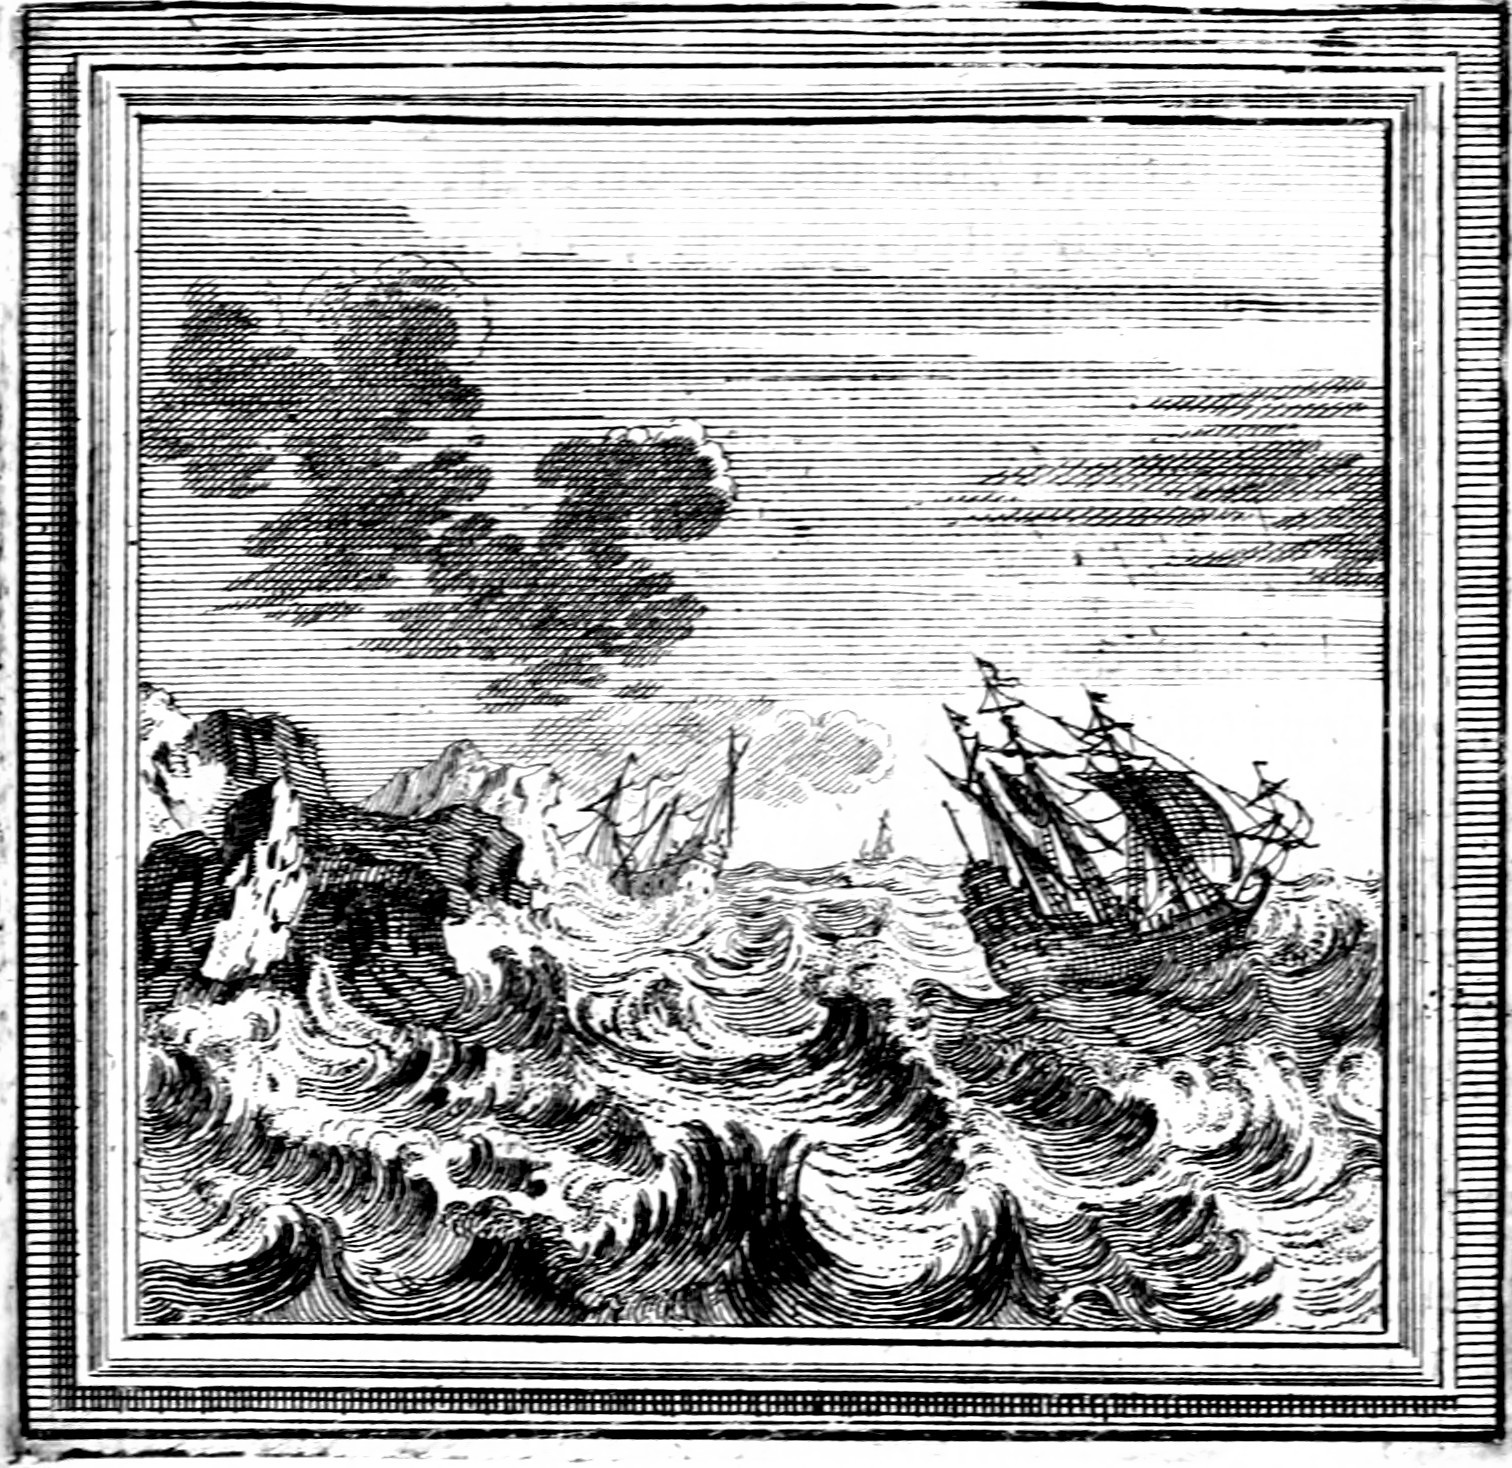
\includegraphics[width=0.7\textwidth]{images/brev11.png}
\end{center}

\breakpage